%
% teil3.tex -- Beispiel-File für Teil 3
%
% (c) 2020 Prof Dr Andreas Müller, Hochschule Rapperswil
%
% !TEX root = ../../buch.tex
% !TEX encoding = UTF-8
%
\section{JPEG Kompression
\label{jpeg:section:kompjpeg}}
\rhead{JPEG Kompression}
Um Bilder mit der DCT transformieren zu können, ist eine Vorverarbeitung nötig. 
in der Vorverarbeitung wird die Farbraumumrechnung um eine bessere Kompression zu erreichen.
Zudem wird das ganze Bild in \(8\times8\) Pixelblöcke unterteilt, da die zweidimensionale DCT damit arbeitet.

\subsection{Farbraumumrechnung
\label{jpeg:subsection:farbraumumrechnung}}
Ein weit verbreiteter Farbmodell ist das Rot-Grün-Blau-Modell (RGB), dabei wird eine Pixelfarbe mit einem Rot-, Grün- und Blauwert additive erzeugt.

Beim JPEG-Standart wechselt man die Basis, in der die Farben dargestellt werden und benutzt statt RGB das YCbCr-Modell.
In diesem Modell werden die Helligkeit (Luminaz Y), sowie die Farbigkeit (Chrominanz).
\(C_b\) von Grau in Richtung Blau/Gelb und \(C_r\) von Grau nach Rot/Türkis.

Die Transformation wird gemacht, weil unsere Augen Empfindlicher sind auf Helligkeitsunterschiede, als auf Farbunterschiede.
Damit lassen sich, nach einer DCT, die Koeffizienten aus den \(C_b\) und \(C_r\) Matrizen stärker Quantisieren als die in der Y Matrix.
Der beschriebene Frabraum wechsel lässt sich
\begin{equation}
    \begin{pmatrix}
        Y\\
        C_b\\
        C_r\\
    \end{pmatrix}
    \thickapprox
    \begin{pmatrix}
        0\\
        128\\
        128\\
    \end{pmatrix}
    +
    \begin{pmatrix}
        0.299 & 0.587 & 0.114\\
        -0.168736 & -0.331264 & 0.5\\
        0.5 & -0.418688 & -0.081312\\
    \end{pmatrix}
    \cdot
    \begin{pmatrix}
        R\\
        G\\
        B\\
    \end{pmatrix}
    \label{jpeg:equationfrab}
\end{equation}
berechnen.
Durch begrenzte Rechengenauigkeit und Rundungsfehler entstehen hier Datenverluste.

\subsection{Tiefpassfilter und Unterabtastung
\label{jpeg:subsection:tiefpass}}

\begin{figure}
    \centering
    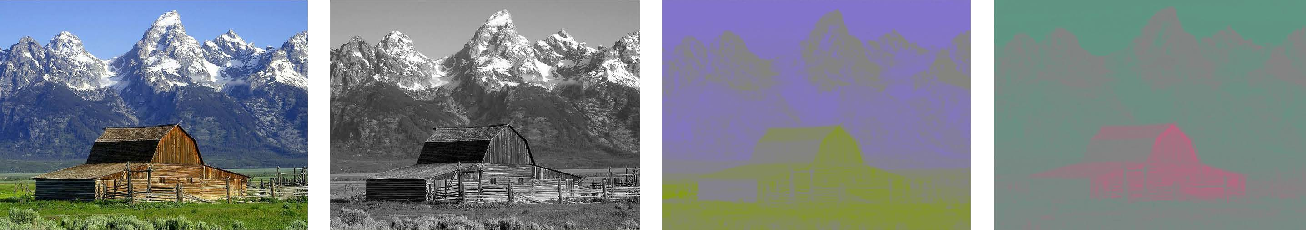
\includegraphics[width=\linewidth]{papers/jpeg/pictures/ycbcr.pdf}
    \caption{Von links Original, Luminanz, Chrominanz Blau/Gelb und Rot/Türkis
        \label{jpeg:fig:ycbcr}}
\end{figure}

Im Abschnitt \ref{jpeg:subsection:farbraumumrechnung} wurde beschrieben, dass die Farbauflösung der \(C_b\) und \(C_r\) für Menschen deutlich geringer ist wie in Abb. \ref{jpeg:fig:ycbcr} ersichtlich.
Dazu werden sie Tiefpass gefiltert, zudem üblicherweise vertikal und horizontal um den Faktor 2 Unterabgetastet, was einer 4 fachen Datenreduktion entspricht.

\subsection{Tiling
\label{jpeg:subsection:tiling}}
Beim Tiling wird das Bild in jeweils \(8\times8\) Pixel grosse Blöcke unterteilt.
Da normalerweise die Seitenlängen eines Bildes sich nicht durch 8 teilen lässt, werden die Restlichen Zeilen bzw. Spalten jeweils aufgefüllt.
Wie das auffüllen geschieht ist im JPEG-Standard nicht festgelegt, es wird jedoch die letzte Pixel-Zeile oder -Spalte jeweils sooft zu wiederholen bis es aufgeht.
Wie in Abb. \ref{jpeg:fig:tiling} ersichtlich.
Auf den einzelnen Blöcken wird nun die DCT angewendet.

\begin{figure}
    \centering
    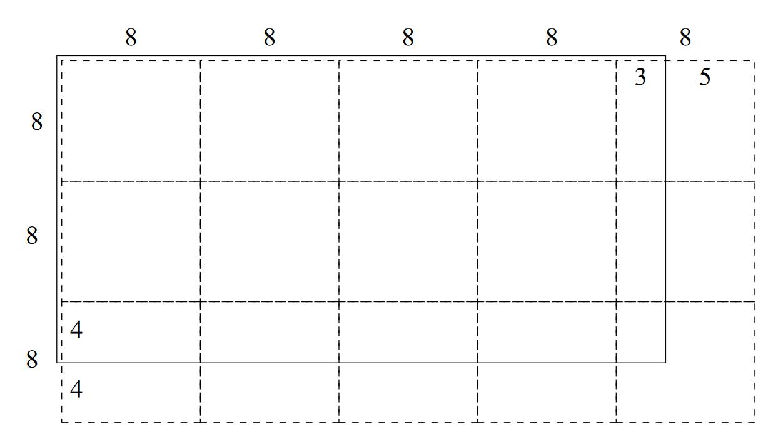
\includegraphics[width=90mm]{papers/jpeg/pictures/unterteilung.pdf}
    \caption{Bildeinteilung und Erweiterung
        \label{jpeg:fig:tiling}}
\end{figure}


\subsection{Quantisierung
\label{jpeg:subsection:quantisierung}}
Bei allen verlustbehafteten Komprimierungsverfahren entsteht die eigentliche Datenreduktion erst bei der Quantisierung.
Dazu werden die Koeffizienten aus der DCT Matrix mit einer Quantisierungsmatrix elementweise dividiert und auf den nächsten ganzzahligen Wert gerundet.
Diese ist für die Qualität und der Menge der reduzierten Daten verantwortlich.
\begin{equation}
    F^Q(x,y)
    =
    round \left(
    \frac{F(x,y)}{Q(x,y)}
    \right)
\end{equation}
dabei ist \(F^Q\) die resultierende Matrix, \(F\) ist der transformierte Pixelblock und \(Q\) die Quantisierungsmatrix.
Bei diesem Schritt findet die Irrelevanzreduktion statt.

Das Auge ist empfindlicher auf hohe Farbunterschiede von benachbarten Pixel, das sind die tiefen Frequenzen in der DCT Matrix.
Daher werden diese weniger Reduziert als die hohen, man sollte dafür eine optimale Tabelle verwenden.

Da der JPEG-Standard das nicht vorgibt, muss die verwendete Tabelle im Header des Files mit abgelegt werden.
In Tabelle \ref{jpeg:tab:quant} ist eine gängige für die Luminanz und eine für die Chrominanzen ersichtlich.

\begin{table}
    \centering
    \begin{tabularx}{0.47\linewidth}{|X|X|X|X|X|X|X|X|}
        \hline
        16 & 11 & 10 & 16 & 24  & 40 & 51 & 61    \\ \hline
        12 & 12 & 14 & 19 & 26  & 58 & 60 & 55    \\ \hline
        14 & 13 & 16 & 24 & 40  & 57 & 69 & 56    \\ \hline
        14 & 17 & 22 & 29 & 51  & 87 & 80 & 62    \\ \hline
        18 & 22 & 37 & 56 & 68  & 109 & 103 & 77  \\ \hline
        24 & 35 & 55 & 64 & 81  & 104 & 113 & 92  \\ \hline
        49 & 64 & 78 & 87 & 103 & 121 & 120 & 101 \\ \hline
        72 & 72 & 95 & 98 & 112 & 100 & 103 & 99  \\ \hline        
    \end{tabularx}
    \qquad
    \begin{tabularx}{0.47\linewidth}{|X|X|X|X|X|X|X|X|}
        \hline
        17 & 18 & 24 & 47 & 99 & 99 & 99 & 99  \\ \hline
        18 & 21 & 26 & 66 & 99 & 99 & 99 & 99  \\ \hline
        24 & 26 & 56 & 99 & 99 & 99 & 99 & 99  \\ \hline
        47 & 66 & 99 & 99 & 99 & 99 & 99 & 99  \\ \hline
        99 & 99 & 99 & 99 & 99 & 99 & 99 & 99  \\ \hline
        99 & 99 & 99 & 99 & 99 & 99 & 99 & 99  \\ \hline
        99 & 99 & 99 & 99 & 99 & 99 & 99 & 99  \\ \hline
        99 & 99 & 99 & 99 & 99 & 99 & 99 & 99  \\ \hline  	  
    \end{tabularx}
    \caption{Beispiel Quantisierungstabelle für Luminanz (links) und Chominanzen
        \label{jpeg:tab:quant}}
\end{table}

\subsection{Umsortierung und Differenzkodierung
\label{jpeg:subsection:umsortierung}}
Die 64 Koeffizienten des Pixelblocks werden nach der Quantisierung im Zig-Zag Muster wie ABB. \ref{jpeg:fig:zigzag} zeigt sortiert.
Die linke obere Ecke ist der Gleichanteil (DC-Wert), das ist die mittlere Helligkeit des Blocks.
Die Koeffizienten mit hohem Wert (die kleinen Frequenzen) stehen nun am Anfang und die kleine weiter hinten.
Je stärker quantisiert wurde desto mehr nullen sind am Ende, was für eine Lauflängenkodierung optimal ist.

\begin{figure}
    \centering
    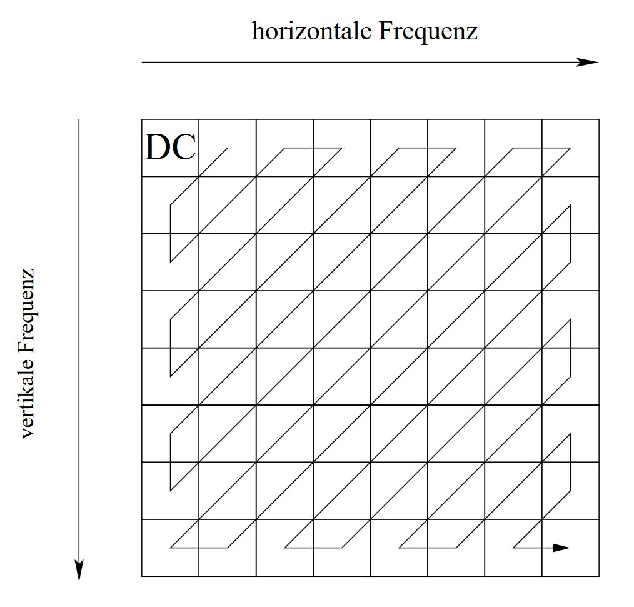
\includegraphics[width=75mm]{papers/jpeg/pictures/zigzag.pdf}
    \caption{Zig-Zag abtastung der Koeffizienten
        \label{jpeg:fig:zigzag}}
\end{figure}

Zudem wird der DC-Wert noch mit dem Block links davon jeweils differenziell kodiert, damit man weiss wie die einzeln transformierten und quantisierten Blöcke zusammenhängen.
Wobei der erste Block mit dem dazugehörigen DC-Wert anfängt
